% fig-crcbaseline: 3-panel expanded gate vs CRC comparison
% Data: R/crcbaseline_panel_[abc].csv → out/crcbaseline-panel-[abc].tex
%
% Chrome (axis-relative), shared:
%   legend @ 1.14  — just above the title row / axis north
%   title  @ 1.02  — tight to the axis top; panel letters on this row
%                    in the left gutter so they never meet the legend
\documentclass[border=2pt]{standalone}
% inspect_style.tex: Shared style definitions for all Inspect figures
% Enforces uniform fonts, colors, and panel label positioning

\usepackage[T1]{fontenc}
\usepackage{lmodern}  % Latin Modern for Type 1 fonts
\usepackage{amssymb}  % \blacksquare for shared legends
\usepackage{pgfplots}
\usepackage{pgfplotstable}
\pgfplotsset{compat=1.18}

% Color palette (Okabe-Ito colorblind-safe, print-safe)
% -- Backbones (used wherever PatchCore vs Dinomaly are distinguished)
\definecolor{cPatchcore}{HTML}{0072B2}   % blue
\definecolor{cDinomaly}{HTML}{D55E00}    % vermillion
% -- Decision classes / gates
\definecolor{cAccept}{HTML}{009E73}      % green
\definecolor{cDefer}{HTML}{E69F00}       % orange
\definecolor{cReject}{HTML}{D55E00}      % red
\definecolor{cControl}{HTML}{56B4E9}     % light blue
\definecolor{cTransfer}{HTML}{CC79A7}    % pink
% -- Benchmarks (canonical palette; used wherever MVTec/VisA/MPDD are
%    distinguished, so benchmark colouring is uniform across all figures and
%    never collides with the backbone blue/vermillion above)
\definecolor{cMVTecAD}{HTML}{0072B2}     % blue
\definecolor{cVisA}{HTML}{E69F00}        % orange
\definecolor{cMPDD}{HTML}{009E73}        % green

% Typography defaults
\newcommand{\figfont}{\fontsize{8}{9.5}\selectfont}
\newcommand{\axislabelfont}{\fontsize{9}{10}\selectfont}
\newcommand{\titlefont}{\fontsize{9}{10}\selectfont}
\newcommand{\tickfont}{\fontsize{7}{8}\selectfont}
\newcommand{\panellabelfont}{\fontsize{9}{10}\selectfont\bfseries}

% Panel label OUTSIDE the axis (axis clip would otherwise swallow it).
% Usage after \end{axis}: \panellabel{axname}{a}
% Parked in the left gutter at the top of the axis frame — NOT on the
% title baseline — so titles can stay truly centered over the plot box.
\newcommand{\panellabel}[2]{%
  \node[anchor=south east, font=\panellabelfont, inner sep=0.5pt]
    at ([xshift=-8pt, yshift=7pt] #1.north west) {\textbf{#2}};%
}

% Standard axis styles. Titles centered above the plot box only.
\pgfplotsset{
  inspect/centertitle/.style={
    title style={at={(0.5,1.10)}, anchor=south, font=\titlefont},
  },
  inspect default/.style={
    axis x line=bottom,
    axis y line=left,
    xlabel style={font=\axislabelfont},
    ylabel style={font=\axislabelfont},
    inspect/centertitle,
    x tick label style={font=\tickfont},
    y tick label style={font=\tickfont},
    legend style={font=\tickfont, draw=none, fill=none},
  }
}


\definecolor{cEscaped}{HTML}{0072B2}
\definecolor{cFalseReject}{HTML}{D55E00}
\definecolor{cDeferral}{HTML}{009E73}

% Letter on the title row, parked in the left gutter (south-east → sits left of NW).
\newcommand{\crclabel}[2]{%
  \node[anchor=south east, font=\panellabelfont, inner sep=0.5pt]
    at ([xshift=-16pt, yshift=11pt] #1.north west) {\textbf{#2}};%
}

\begin{document}
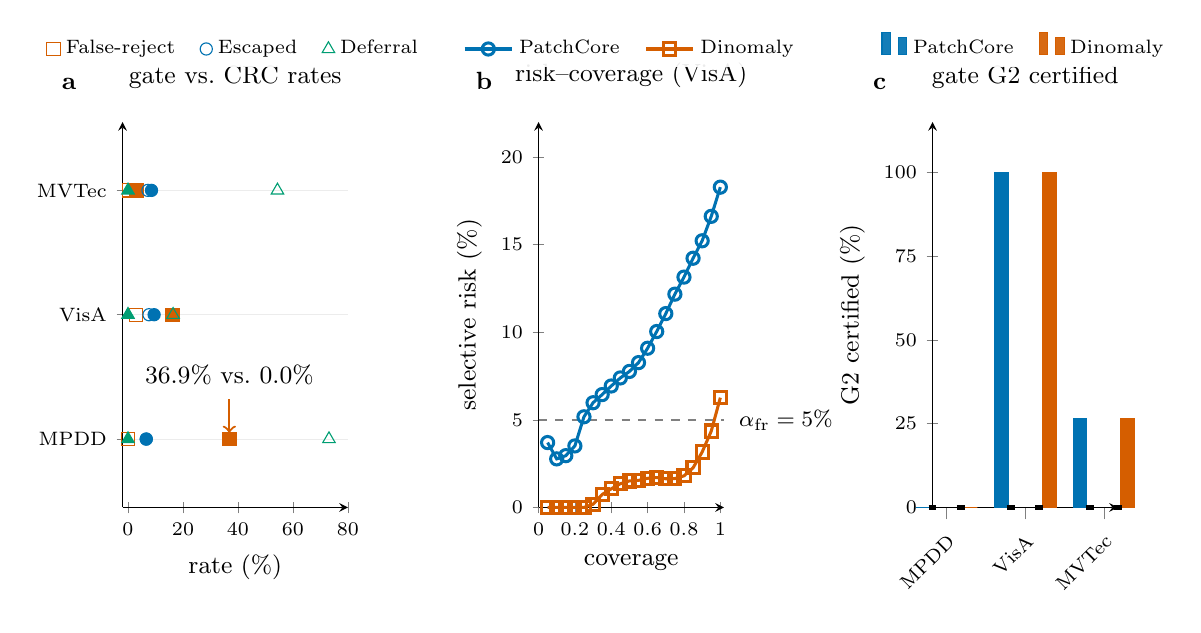
\begin{tikzpicture}[font=\figfont]

\pgfplotsset{
  crc/title near axis/.style={
    title style={at={(0.5,1.02)}, anchor=south, font=\titlefont},
  },
  crc/legend above/.style={
    legend style={
      at={(0.5,1.14)}, anchor=south,
      legend columns=-1, font=\tickfont, draw=none,
      fill=white, fill opacity=0.92, text opacity=1,
      inner sep=1.5pt, /tikz/every even column/.append style={column sep=7pt},
    },
  },
}

% Panel a: gate (hollow) vs CRC (filled) rates — title matches caption intent.
\begin{axis}[
  inspect default,
  name=axa, width=1.75in, height=2.55in, at={(0.50in,0)},
  xmin=-2, xmax=80, ymin=-0.55, ymax=2.55,
  xlabel={rate (\%)},
  ytick={0,1,2}, yticklabels={MPDD, VisA, MVTec},
  ymajorgrids, grid style={gray!15},
  crc/title near axis,
  crc/legend above,
  title={gate vs.\ CRC rates},
  clip=false,
]
% generated by process_crcbaseline.R
\addplot[cFalseReject, only marks, mark=square*, mark size=2.4pt, forget plot] coordinates {(36.8523,0) (16.2399,1) (3.0570,2)};
\addplot[cFalseReject, only marks, mark=square, draw=cFalseReject, mark size=2.4pt] coordinates {(0.0000,0) (2.9576,1) (0.4560,2)};
\addlegendentry{False-reject}
\addplot[cEscaped, only marks, mark=*, mark size=2.2pt, forget plot] coordinates {(6.6308,0) (9.4917,1) (8.5476,2)};
\addplot[cEscaped, only marks, mark=o, mark size=2.2pt] coordinates {(6.6308,0) (7.6367,1) (7.2514,2)};
\addlegendentry{Escaped}
\addplot[cDeferral, only marks, mark=triangle*, mark size=2.6pt, forget plot] coordinates {(0.0000,0) (0.0000,1) (0.0000,2)};
\addplot[cDeferral, only marks, mark=triangle, draw=cDeferral, mark size=2.6pt] coordinates {(73.0911,0) (16.3945,1) (54.3573,2)};
\addlegendentry{Deferral}
\draw[cFalseReject, thick, ->] (axis cs:36.8523,0.32) -- (axis cs:36.8523,0.05);
\node[font=\axislabelfont, text=black, anchor=south] at (axis cs:36.8523,0.36) {$36.9\%$ vs.\ $0.0\%$};

\end{axis}
\crclabel{axa}{a}

% Panel b: selective risk-at-coverage on VisA (not “VisA” alone).
\begin{axis}[
  inspect default,
  name=axb, width=1.55in, height=2.55in, at={(2.58in,0)},
  xmin=0, xmax=1.02, ymin=0, ymax=22,
  xlabel={coverage},
  ylabel={selective risk (\%)},
  crc/title near axis,
  crc/legend above,
  title={risk--coverage (VisA)},
  clip=false,
]
% generated by process_crcbaseline.R
\addplot[cPatchcore, mark=o, line width=1.1pt, mark size=2.2pt] coordinates {(0.0500,3.7037) (0.1000,2.7726) (0.1500,2.9557) (0.2000,3.5120) (0.2500,5.1737) (0.3000,5.9766) (0.3500,6.4414) (0.4000,6.9316) (0.4500,7.3922) (0.5000,7.7634) (0.5500,8.2661) (0.6000,9.0881) (0.6500,10.0398) (0.7000,11.0642) (0.7500,12.1735) (0.8000,13.1470) (0.8500,14.2236) (0.9000,15.2187) (0.9500,16.6148) (1.0000,18.2810)};
\addlegendentry{PatchCore}
\addplot[cDinomaly, mark=square, line width=1.1pt, mark size=2.2pt] coordinates {(0.0500,0.0000) (0.1000,0.0000) (0.1500,0.0000) (0.2000,0.0000) (0.2500,0.0000) (0.3000,0.1848) (0.3500,0.7392) (0.4000,1.0628) (0.4500,1.3552) (0.5000,1.5157) (0.5500,1.5457) (0.6000,1.6636) (0.6500,1.7065) (0.7000,1.6372) (0.7500,1.6511) (0.8000,1.8022) (0.8500,2.2619) (0.9000,3.1629) (0.9500,4.3580) (1.0000,6.2662)};
\addlegendentry{Dinomaly}
\draw[gray, dashed, line width=0.9pt] (axis cs:0,5.0000) -- (axis cs:1.02,5.0000);
\node[anchor=west, font=\figfont, text=black] at (axis cs:1.05,5.0000) {$\alpha_{\mathrm{fr}}=5\%$};

\end{axis}
\crclabel{axb}{b}

% Panel c: bars = dual-gate G2 cert.\ per backbone; dashed ticks at 0 = CRC.
\begin{axis}[
  inspect default,
  name=axc, width=1.55in, height=2.55in, at={(4.55in,0)},
  ymin=0, ymax=115, ytick={0,25,50,75,100},
  ylabel={G2 certified (\%)},
  xtick={0,1,2}, xticklabels={MPDD, VisA, MVTec},
  x tick label style={font=\tickfont, rotate=45, anchor=north east},
  ybar=2pt, bar width=5pt,
  crc/title near axis,
  crc/legend above,
  title={gate G2 certified},
  clip=false,
]
% generated by process_crcbaseline.R
\addplot[cPatchcore, fill=cPatchcore] coordinates {(-0.1800,0.0000) (0.8200,100.0000) (1.8200,26.6667)};
\addlegendentry{PatchCore}
\addplot[cDinomaly, fill=cDinomaly] coordinates {(0.1800,0.0000) (1.1800,100.0000) (2.1800,26.6667)};
\addlegendentry{Dinomaly}

\draw[black, dashed, line width=1.5pt] (axis cs:-0.23,0) -- (axis cs:-0.13,0);
\draw[black, dashed, line width=1.5pt] (axis cs:0.13,0) -- (axis cs:0.23,0);
\draw[black, dashed, line width=1.5pt] (axis cs:0.77,0) -- (axis cs:0.87,0);
\draw[black, dashed, line width=1.5pt] (axis cs:1.13,0) -- (axis cs:1.23,0);
\draw[black, dashed, line width=1.5pt] (axis cs:1.77,0) -- (axis cs:1.87,0);
\draw[black, dashed, line width=1.5pt] (axis cs:2.13,0) -- (axis cs:2.23,0);
\end{axis}
\crclabel{axc}{c}

\end{tikzpicture}
\end{document}
